\let\negmedspace\undefined
\let\negthickspace\undefined
\documentclass[journal]{IEEEtran}
\usepackage[a5paper, margin=10mm, onecolumn]{geometry}
\usepackage{lmodern} % Ensure lmodern is loaded for pdflatex
\usepackage{tfrupee} % Include tfrupee package

\setlength{\headheight}{1cm} % Set the height of the header box
\setlength{\headsep}{0mm}     % Set the distance between the header box and the top of the text

\usepackage{gvv-book}
\usepackage{gvv}
\usepackage{cite}
\usepackage{amsmath,amssymb,amsfonts,amsthm}
\usepackage{algorithmic}
\usepackage{graphicx}
\usepackage{textcomp}
\usepackage{xcolor}
\usepackage{txfonts}
\usepackage{listings}
\usepackage{enumitem}
\usepackage{mathtools}
\usepackage{gensymb}
\usepackage{comment}
\usepackage[breaklinks=true]{hyperref}
\usepackage{tkz-euclide} 
\usepackage{listings}
 \usepackage{gvv}                                        
\def\inputGnumericTable{}                                 
\usepackage[latin1]{inputenc}                                
\usepackage{color}                                            
\usepackage{array}                                            
\usepackage{longtable}                                       
\usepackage{calc}                                             
\usepackage{multirow}                                         
\usepackage{hhline}                                           
\usepackage{ifthen}                                           
\usepackage{lscape}
\begin{document}

\bibliographystyle{IEEEtran}


\title{2.4.16}
\author{EE25BTECH11021 - Dhanush Sagar
}
% \maketitle
% \newpage
% \bigskip
{\let\newpage\relax\maketitle}

\renewcommand{\thefigure}{\theenumi}
\renewcommand{\thetable}{\theenumi}
\setlength{\intextsep}{10pt} % Space between text and floats


\numberwithin{equation}{enumi}
\numberwithin{figure}{enumi}
\renewcommand{\thetable}{\theenumi}


\textbf{Question} \\
Verify the following:\\  
(a) $(0,7,-10), (1,6,-6)$ and $(4,9,-6)$ are the vertices of an isosceles triangle.  \\
(b) $(0,7,10), (-1,6,6)$ and $(-4,9,6)$ are the vertices of a right-angled triangle.  


\textbf{Solution a}\\
% ---------- Part (a) ----------
\textbf{Property:} In an isosceles triangle, the perpendicular bisector of a side passes through the opposite vertex.

\begin{align}
\vec{A} = \myvec{0\\7\\-10},  
\vec{B} = \myvec{1\\6\\-6},  
\vec{C} = \myvec{4\\9\\-6}
\end{align}
\text{Midpoint of side } AC: 
\begin{align}
 \vec{M} = \frac{\vec{A}+\vec{C}}{2} 
= \frac{\myvec{0\\7\\-10}+\myvec{4\\9\\-6}}{2} 
= \myvec{2\\8\\-8}
\end{align}
\text{Direction vector of side } AC: 
\begin{align}
 \vec{C}-\vec{A} = \myvec{4\\9\\-6}-\myvec{0\\7\\-10} 
= \myvec{4\\2\\4}
\end{align}
\text{Vector from midpoint to } B:
\begin{align}
\vec{B}-\vec{M} = \myvec{1\\6\\-6}-\myvec{2\\8\\-8} 
= \myvec{-1\\-2\\2}
\end{align}
\begin{align}
(\vec{C}-\vec{A})^\top(\vec{B}-\vec{M}) 
= \myvec{4&2&4}\myvec{-1\\-2\\2} = -4-4+8=0
\end{align}
\begin{align*}
 \vec{B} \text{ lies on the perpendicular bisector of side } AC.\\
 \therefore AB = BC \implies \triangle ABC \text{ is isosceles.}
\end{align*}
\textbf{Solution b}\\
\textbf{Property:} If two sides of a triangle are perpendicular, then the included angle is a right angle.
\begin{align}
\vec{A} = \myvec{0\\7\\10},  
\vec{B} = \myvec{-1\\6\\6},  
\vec{C} = \myvec{-4\\9\\6}
\end{align}
\begin{align}
\vec{A}-\vec{B} = \myvec{0\\7\\10}-\myvec{-1\\6\\6} 
= \myvec{1\\1\\4}
\end{align}
\begin{align}
\vec{C}-\vec{B} = \myvec{-4\\9\\6}-\myvec{-1\\6\\6} 
= \myvec{-3\\3\\0}
\end{align}
\begin{align}
(\vec{A}-\vec{B})^\top(\vec{C}-\vec{B}) 
= \myvec{1&1&4}\myvec{-3\\3\\0} = -3+3+0=0
\end{align}
\begin{align*}
\implies \vec{A}-\vec{B} \perp \vec{C}-\vec{B}  \Rightarrow  
\triangle ABC \text{ is right-angled at } B.
\end{align*}
\begin{figure}[H]
    \centering
    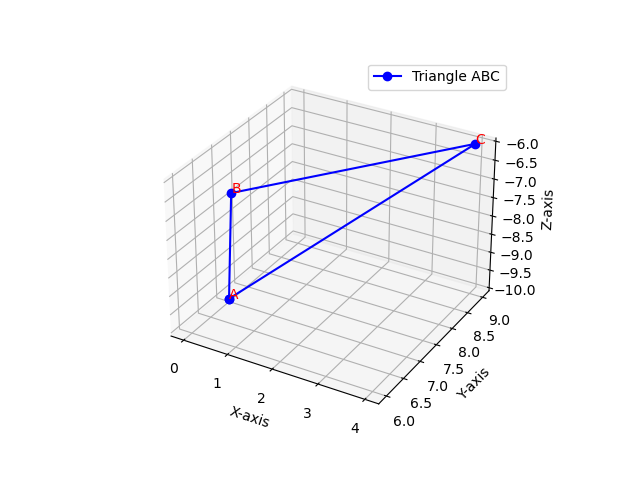
\includegraphics[width=0.8\columnwidth]{figs/fig1.png}
    \caption{isosceles triangle(a)}
    \label{fig:fig1}
\end{figure}
\begin{figure}[H]
    \centering
    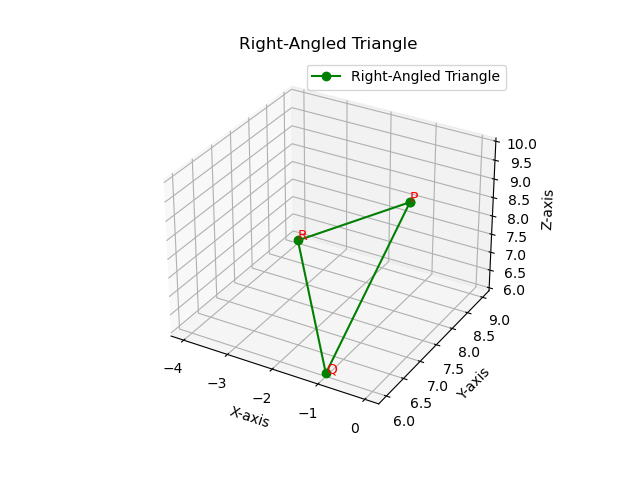
\includegraphics[width=0.8\columnwidth]{figs/fig2.png}
    \caption{}
    \label{fig:fig2}
\end{figure}
\end{document}

